% Created 2013-06-02 Sun 21:53
\documentclass[11pt,a4paper]{article}
\usepackage[T1]{fontenc}
\usepackage{float}
\usepackage{fontspec}
\usepackage{graphicx}
\defaultfontfeatures{Mapping=tex-text}
\setmainfont{DejaVu Sans}
\setmonofont[Scale=0.8]{FreeMono}
\usepackage{geometry}
\geometry{a4paper, textwidth=6.5in, textheight=10in,
            marginparsep=7pt, marginparwidth=.6in}
\usepackage[usenames,dvipsnames]{xcolor}
\usepackage[bookmarks, colorlinks, breaklinks]{hyperref}
\hypersetup{linkcolor=black, citecolor=blue,filecolor=black,urlcolor=MidnightBlue}
\pagestyle{empty}
\usepackage{amsmath}
\author{Maria Karageorgiou, Chris Perivolaropulos}
\date{\today}
\title{Profapp report}
\hypersetup{
  pdfkeywords={},
  pdfsubject={},
  pdfcreator={Emacs 24.3.1 (Org mode 8.0.3)}}
\begin{document}

\maketitle
\tableofcontents


\section{Πριγραφή της Βάσης}
\label{sec-1}
Η βάση δεδομένων περιγραφει τη συσχέτιση φοιτητών με μαθηματα
ανά έτος, διαγωνίσματα και τους αντίστοιχους βαθμούς. Σκοπός ειναι η
διευκόλυνση ενός καθηγητη να οργανώσει τα μαθήματα του. Στη βαση
εχουμε πίνακες βαθμών, φοιτητών, διαγωνισμάτων και μαθημάτων ανα
έτος. Κάθε βαθμός αντιστοιχεί σε ένα φοιτητή και σε ενα
διαγώνισμα το οποιο αντιστοιχεί σε ενα μάθημα στο οποίο είναι
εγγεγραμένοι φοιτητές.

Παρακάτω φαίνεται το εννοιολογικό μοντέλο της βάσης.

Περιγραφή:

Υπάρχει η οντότητα "Φοιτητής" με τα εξής γνωρίσματα: Αριθμός
μητρώου, επώνυμο, όνομα, ετός εγγραφής στη σχολή, εξάμηνο φοίτησης
και ένα γνώρισμα που δηλώνει αν είναι προπτυχιακός ή οχι. Ο φοιτητής
γράφεται σε διάφορα μαθήματα και παίρνει βαθμούς στα αντίστοιχα
διαγωνίσματα που έδωσε.

Άλλη οντότητα είναι το "Μάθημα ανά έτος" με μοναδικά γνωρίσματα το
όνομά του και το έτος που διδάχθηκε κάθε φορά. Έχει διάφορα
διαγωνίσματα και φοιτητές εγγεγραμμένους.

Επίσης έχουμε την οντότητα "Διαγωνίσματα" με γνωρίσματα τον τύπο του
διαγωνίσματος (final, midterm, excercises, test), το ποσοστό με το
οποίο συντελεί στον τελικό βαθμό του αντίστοιχου μαθήματος και ένα
αρχείο με τα θέματα. Το κάθε διαγώνισμα ανήκει υποχρεωτικά σε ένα
μάθημα συγκεκριμένου έτους και έχει βαθμούς φοιτητών.

Τέλος είναι και η οντότητα "Βαθμοί" με μοναδικό γνώρισμα τον βαθμό
που πήρε συγκεκριμένος φοιτητής σε συγκεκριμένο διαγώνισμα.

\begin{figure}[H]
\centering
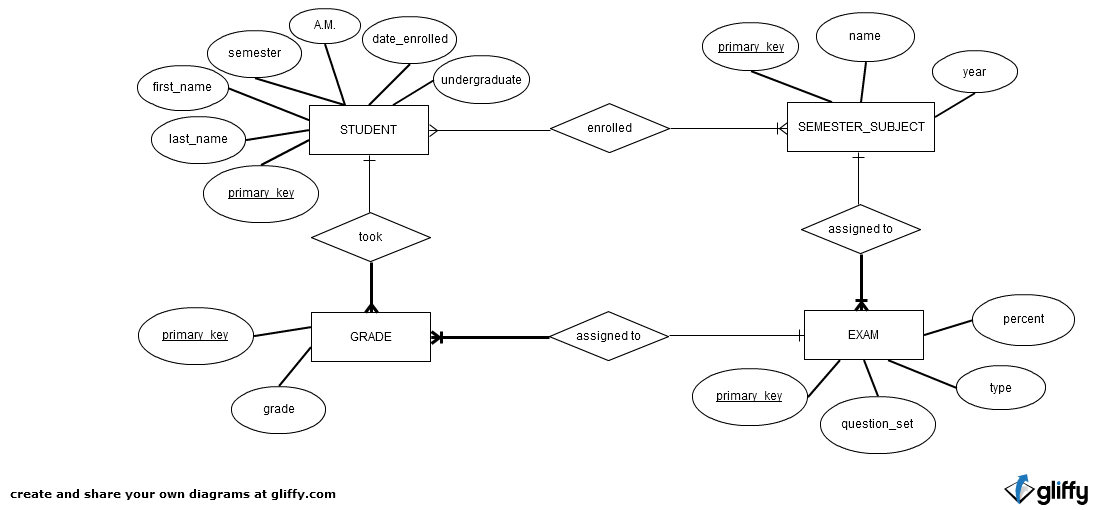
\includegraphics[width=.9\linewidth]{./profapp.png}
\caption{\label{fig:profapp_erd.png}Το λογικό διάγραμμα της βάσης.}
\end{figure}


\begin{figure}[H]
\centering
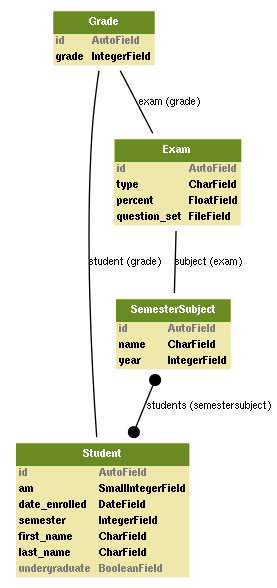
\includegraphics{./profapp_erd.png}
\caption{\label{fig:profapp_erd.png}Το ERD διάγραμμα της βάσης.}
\end{figure}
\newpage
\section{Δημιουργία Βάσης}
\label{sec-2}
Η SQL που παράγει τη βάση:

\begin{verbatim}
BEGIN;
CREATE TABLE "profapp_student" (
    "id" integer NOT NULL PRIMARY KEY,
    "am" smallint NOT NULL UNIQUE,
    "date_enrolled" date NOT NULL,
    "semester" integer NOT NULL,
    "first_name" varchar(100) NOT NULL,
    "last_name" varchar(100) NOT NULL,
    "undergraduate" bool NOT NULL
)
;
CREATE TABLE "profapp_semestersubject_students" (
    "id" integer NOT NULL PRIMARY KEY,
    "semestersubject_id" integer NOT NULL,
    "student_id" integer NOT NULL REFERENCES "profapp_student" ("id"),
    UNIQUE ("semestersubject_id", "student_id")
)
;
CREATE TABLE "profapp_semestersubject" (
    "id" integer NOT NULL PRIMARY KEY,
    "name" varchar(100) NOT NULL,
    "year" integer NOT NULL
)
;
CREATE TABLE "profapp_exam" (
    "id" integer NOT NULL PRIMARY KEY,
    "subject_id" integer NOT NULL REFERENCES "profapp_semestersubject" ("id"),
    "type" varchar(15) NOT NULL,
    "percent" real NOT NULL,
    "question_set" varchar(100) NOT NULL
)
;
CREATE TABLE "profapp_grade" (
    "id" integer NOT NULL PRIMARY KEY,
    "student_id" integer NOT NULL REFERENCES "profapp_student" ("id"),
    "grade" integer NOT NULL,
    "exam_id" integer NOT NULL REFERENCES "profapp_exam" ("id")
)
;

COMMIT;
\end{verbatim}
\section{Εφαρμογή profapp}
\label{sec-3}
Τη βάση αυτη διαχειρίζεται μια εφαρμογή που ονομάσαμε profapp η
οποία χτίστηκε με το προγραμματιστικό περιβάλλον(framework) django
και προορίζεται για online χρήση. Για οδηγίες εγκατάστασης δείτε το
\href{http://github.com/fakedrake/django-profapp}{github} της εφαρμογής για λεπτομέρειες εγκατάστασης και
χρήσης. Μερικα απο τα features που συμπεριλάβαμε στην alpha εκδοση:

\begin{itemize}
\item εμφάνιση των μοντελων με λεπτομερειες/σε λιστα
\item Δημιουργία/διαγραφη/επεξεργασία μοντέλων
\item Εύκολη πλοήγηση στην εφαρμογή
\item Ομορφος σχεδιασμός με χρήση του bootstrap
\end{itemize}
\section{Οργάνωση του project}
\label{sec-4}
\subsection{Χρήστος Περιβολαρόπουλος}
\label{sec-4-1}
\begin{itemize}
\item Επιλογή και στήσιμο του βασικού toolchain και των βιβλιοθκών που
χρησιμοποιήθηκαν.
\item Template tags για εμφάνιση των ερωτημάτων SQL.
\item Βασικός σκελετός του project
\item Views
\item Debugging
\end{itemize}
\subsection{Μαρία Καραγεωρίου}
\label{sec-4-2}
\begin{itemize}
\item Templates
\item ERD
\item Views
\item Debugging
\end{itemize}
% Emacs 24.3.1 (Org mode 8.0.3)
\end{document}
